\documentclass{article} % For LaTeX2e
\usepackage{iclr2027_conference,times}

% Optional math commands from https://github.com/goodfeli/dlbook_notation.
\input{math_commands.tex}

\usepackage{graphicx}
\usepackage{float}
\usepackage{url}
% Load hyperref after float so caption anchors do not create an empty line.
\usepackage{hyperref}

\title{Formatting Instructions for ICLR 2027 \\ Conference Submissions}

% Keep this anonymous for double-blind submission. Add author information only
% for the camera-ready version, together with \iclrfinalcopy.
\author{}

\newcommand{\fix}{\marginpar{FIX}}
\newcommand{\new}{\marginpar{NEW}}

%\iclrfinalcopy % Uncomment for camera-ready version, but NOT for submission.
\begin{document}

% Keep natural vertical spacing on pages with large figures; leave spare
% space at the page bottom instead of stretching headings and float gaps.
\raggedbottom

\maketitle

\begin{abstract}
Effective multi-agent interaction requires agents to infer their partners'
preferences and plan actions in light of those inferences. Terminal outcomes,
however, reveal little about where either capability fails. We study inference
and planning in a finite negotiation game with private preferences and mixed
incentives. An oracle computes beliefs and action values under a fixed
reference policy, allowing us to evaluate the two capabilities at the same
decision. Qwen3-4B-Instruct-2507 misreads partner behavior and often chooses
suboptimal actions even when given the correct inference. Replacing its
inference with an oracle judgment changes its choices but does not reliably
improve their value. We then construct \emph{game
slices}, contiguous segments of one or more decisions drawn from deliberately
structured games, and use oracle labels to train action selection, inference,
and planning conditioned on a correct inference. We compare this targeted
training with complete-game self-play and evaluate transfer to meeting
coordination with private calendars. On a 24-game sequential adaptation of
CalBench, joint slice training retains 47 of 72 meetings, compared with 37
for both the unchanged baseline and the self-play model. These results
support controlled games as a means of diagnosing interaction failures and
training capabilities that transfer to more complex coordination.
\end{abstract}

\section{Introduction}
Large language models (LLMs) are increasingly deployed as interacting agents that exchange 
information, negotiate decisions, and coordinate their actions over multiple turns. 
Such multi-agent systems (MAS) promise to combine information and capabilities distributed
across multiple agents, yet recent work has exposed substantial failures that arise 
specifically through interaction. Agents fail to proactively acquire information that 
is available only to others \citep{li2026systematic}, communicate actively without 
converting those exchanges into effective distributed reasoning \citep{zhang2026silobench}, 
and remain unable to coordinate effectively even when relevant information is made 
transparent \citep{yao2026talk}. Broader analyses similarly identify inter-agent failures 
as a distinct source of error beyond mistakes made by individual agents in isolation 
\citep{cemri2025multiagent,anthropic2026multiagent}. These findings raise a basic question: 
what capabilities are missing when individually capable agents fail to interact effectively?

Classical models of interactive decision making provide a principled way to make this question 
more precise. In an interactive POMDP, an agent maintains uncertainty not only over the 
physical environment, but also over models of other agents, and plans its own actions 
with respect to this interactive state \citep{gmytrasiewicz2005ipomdp}. Related work 
on opponent modeling similarly couples inference about another agent with planning a 
response to the inferred model \citep{huang2024hop}. Viewed through this lens, 
effective interaction requires at least two computations: \textbf{interactive-state inference}, 
which construct belief of other agents relevant information, and \textbf{interaction planning}, 
which uses that belief to evaluate what to do next. Importantly, these computations are 
coupled over time. An inferred state changes the value of a interaction action; 
the selected interaction then changes how other agents respond and therefore what 
evidence becomes available for subsequent inference. Established models of multi-agent 
decision making identify these two computations as fundamental components of interaction, 
motivating us to ask whether current LLM agents can reliably perform them together \citep{riemer2025tom}.

How can these capabilities be diagnosed and trained in a controlled way? 
Games provide a natural substrate because their information structure, utilities, legal 
actions, and strategic consequences can be specified and verified exactly. 
Recent work has accordingly used multi-agent games and self-play to train strategic 
or transferable reasoning in LLMs \citep{yuan2026marshal,liu2026spiral,lyu2026gift,he2026stratreasoner}. 
However, these environments are primarily designed around game-level performance rather than 
separate supervision of interactive-state inference and the planning that follows from it. 
Compact self-play games make scalable training possible but often abstract away the 
combination of latent information and heterogeneous incentives, whereas richer social games 
can entangle deduction, communication, deception, commitment and execution within the same 
trajectory \citep{light2023avalonbench}. To obtain precise supervision for the interaction 
structure above, we instead extend an existing commitment-based multi-party negotiation 
game \citep{benac2026benchmark}, which makes the environment becomes incomplete information and mixed incentives. 
Incomplete information makes relevant properties of other agents latent and therefore creates an inference problem, 
while mixed incentives make those inferred properties consequential for planning because the value of an interaction depends on what the other agents know, prefer, or are likely to do. 
Their combination captures an important class of real interactions in which agents act 
on behalf of different principals---for example, coordinating around private scheduling 
constraints \citep{zou2026calbench}, negotiating under asymmetric private objectives \citep{oneill2026cooperate}, 
or interacting repeatedly on behalf of distinct economic interests \citep{li2026emergent}.

Using this controlled setting, we separately diagnose failures in interactive-state inference 
and interaction planning, then construct strategic game slices that provide oracle 
supervision for both. We train on these slices and evaluate whether the resulting 
improvements generalize to unseen strategic configurations and transfer to external 
multi-agent environments. 

Our contributions are threefold:

\begin{itemize}
    \item \textbf{A controlled diagnosis of interactive reasoning in LLM-based MAS.} Grounded in classical interactive decision making, we study interactive-state inference and interaction planning in incomplete-information, mixed-incentive coordination, and separately measure failures in the two while retaining their sequential dependence.
    \item \textbf{A compact game construction for verifiable social-reasoning supervision.} We show how private preferences, consequential commitments, and information-revealing actions can instantiate a practically relevant interactive-decision problem while providing exact latent-state targets and counterfactual action values.
    \item \textbf{Targeted game supervision and transfer.} We construct strategic game slices around diagnosed interaction decisions, use their oracle structure to supervise inference and planning, and test whether the resulting capabilities generalize to unseen strategic configurations and external multi-agent environments.
\end{itemize}


\section{Motivation and Methods}
\subsection{From Interactive Uncertainty to Two Capabilities}
\label{sec:coordination-formulation}

Consider three coding agents working on the same Python backend. In an
Anthropic experiment motivated by behavior observed in deployment, each was
instructed to migrate it to a different language. The agents mistook the resulting interference for deliberate
obstruction and escalated to repeatedly killing competing processes and, in
some runs, revoking one another's access~\citep{anthropic2026multiagent}.
They depended on a usable shared backend, yet pursued incompatible local
objectives without knowing the others' instructions. Such coordination is naturally an interactive partially
observable decision problem.  For agent $i$, an I-POMDP is $\mathcal I_i=\langle IS_i,A,T_i,\Omega_i,O_i,R_i\rangle, IS_i=S\times\prod_{j\neq i}M_j$
where $S$ is the physical state, $M_j$ models agent $j$, $A$ is the joint
action space, and $T_i,O_i,R_i$ specify transition, observation, and
reward~\citep{gmytrasiewicz2005ipomdp}.  Uncertainty therefore covers not only
the world but also others' information, preferences, and policies. This view
underlies opponent modelling and belief-space coordination
\citep{carmel1996opponent,huang2024hop,goel2026bayesian}; the observation--belief--action
links nevertheless remain fragile for LLM agents
\citep{sobotka2026strategic,jha2026modeling}. 
Let $b_t^i\in\Delta(IS_i)$ be agent $i$'s belief after public history $h_t$.
An observation updates it as $b_{t+1}^i=\tau_i(b_t^i,a_t^i,o_{t+1}^i)$, while
an action is selected by belief-conditioned planning: $a_t^{i,*}\in\arg\max_{a\in A_i}\mathbb E\!\left[\sum_{k=t}^{T}\gamma^{k-t}R_i(x_k,a_k)\mid b_t^i,a_t^i=a,\pi_{-i}\right]$.
We call these computations \emph{inference}, which maintains the
part of $b_t^i$ predictive of others, and \emph{planning}, which evaluates
actions under that belief. They form a loop: inference informs an action,
the action determines the next observation, and that observation informs the
next inference. For this distinction to be experimentally useful, the hidden state must be
both inferable and consequential: interaction must provide evidence that
supports a reasonable belief about another agent, and different beliefs must affect the
relative value of available actions. We therefore need decision points at
which evidence, private information, and action consequences are all specified
well enough to evaluate the belief and the choice separately. In the game
below, we operationalize inference with an inference target and planning
with counterfactual action values.

\subsection{Negotiation with Private Preferences and Mixed Incentives}
\label{sec:benac-i}

To make inference and planning separately observable while retaining exact
supervision, we extend the commitment-based negotiation game of
\citet{benac2026benchmark} with private preferences and costly information
gathering. An instance of this game is
\begin{equation}
 \mathcal E=\langle\mathcal N,\mathbf K,\mathcal G,\Gamma,\delta,
 \rho,C_0,\mathcal L,\{\Theta_i\}_{i\in\mathcal N},\mu_0,\mathbf q_0\rangle .
 \label{eq:benac-i-game}
\end{equation}
Here $\mathcal N$ is the player set and $\mathbf K=(K_i)_{i\in\mathcal N}$
gives each player's number of binary commitment coordinates. Each public goal
$g\in\mathcal G$ has a nonempty requirement set
$\Gamma_g\subseteq\{(i,k):i\in\mathcal N,\ 0\leq k<K_i\}$ and a scoring mode
$\delta_g\in\{\mathrm{binary},\mathrm{linear}\}$. The public schedule
$\rho=(\rho_t)_{t=0}^{T-1}$ specifies the proposer at each of $T$ proposal
opportunities, and $\mathcal L$ gives the legal actions at each information
set. The commitment state is $C=(c_{ik})$, with $c_{ik}\in\{0,1\}$; initially
$C_0=0$, and a commitment cannot be withdrawn. Each player privately observes
its preference vector $v_i\in\Theta_i\subseteq\{-1,0,+1\}^{|\mathcal G|}$.
The joint type $v=(v_i)_{i\in\mathcal N}$ is drawn from the common prior
$\mu_0\in\Delta(\prod_{i\in\mathcal N}\Theta_i)$; entries encode
\textsc{Avoid}, \textsc{Neutral}, and \textsc{Want}, respectively.
$\mathbf q_0=(q_{i,0})_{i\in\mathcal N}$ gives the initial investigation
budgets. For any commitment state $C$, goal satisfaction and terminal utility
are
\begin{equation}
 S_g(C)=
 \begin{cases}
 \mathbf 1[\,c_{ik}=1,\ \forall(i,k)\in\Gamma_g\,],&\delta_g=\mathrm{binary},\\
 \dfrac{1}{|\Gamma_g|}\sum_{(i,k)\in\Gamma_g}c_{ik},&\delta_g=\mathrm{linear},
 \end{cases}
 \qquad U_i(C;v_i)=\sum_{g\in\mathcal G}v_{ig}S_g(C).
 \label{eq:benac-i-utility}
\end{equation}
At initialization, the goals, prior, legal-action rules, and proposer schedule are
public, while each player sees only its own sampled preferences; every player
starts with one investigation opportunity ($q_{i,0}=1$). Play follows $\rho$.
At each proposal opportunity, the scheduled player may \textsc{pass}, make a
bilateral \textsc{offer} to a chosen partner, or, if $q_{i,t}>0$, use
\textsc{Investigate}$(j,g)$ to learn $v_{jg}$. Passing leaves commitments
unchanged. Investigation also leaves them unchanged, uses that proposal
opportunity and one unit of budget, and reveals the answer only to the
investigator; the query target is public. An offer specifies new commitments
for the proposer, the partner, or both. The partner immediately chooses
\textsc{accept} or \textsc{reject}: acceptance makes all proposed additions
binding and irreversible, whereas rejection changes no commitments. The
response does not use another proposal opportunity. Play then proceeds to the
next scheduled proposer and ends after the final opportunity, when each
player receives $U_i(C_T;v_i)$. To improve its utility, a player infers
partners' preferences from offers, responses, and any private investigation
answers, then plans whom to approach, what to offer, and whether to accept,
accounting for goals on which preferences align or conflict.

Figure~\ref{fig:game-flow} illustrates these transitions in a
three-player game.
\begin{figure}[H]
\centering
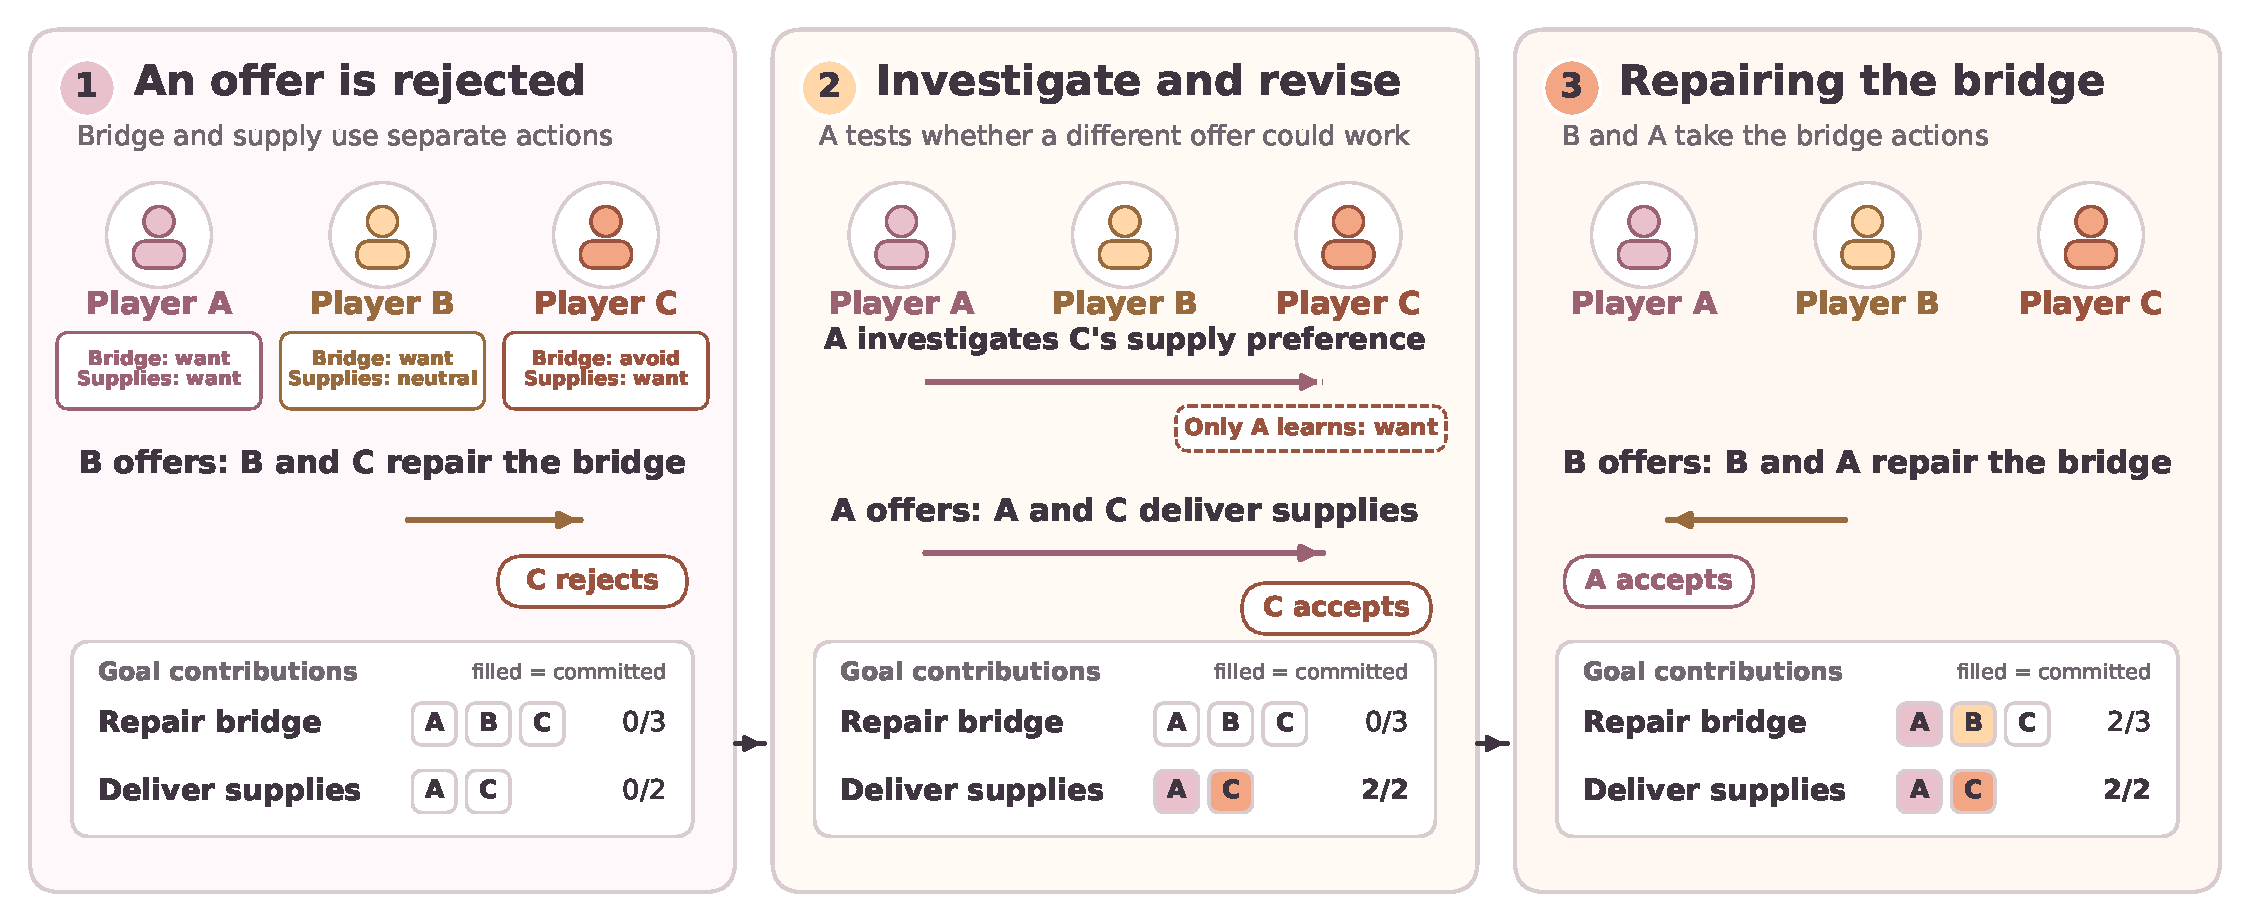
\includegraphics[width=\textwidth]{figures/game_flow.pdf}
\caption{An illustrative three-player negotiation with private preferences
and two linearly scored goals. \emph{Repair bridge} requires distinct bridge
actions from A, B, and C; \emph{Deliver supplies} requires distinct supply
actions from A and C. A filled letter indicates that player's commitment to
that particular goal, and the fractions show goal progress. B first offers
bridge actions to C, who rejects: accepting would leave the bridge at $2/3$
and give C $-2/3$ from a goal it dislikes if play stopped then. A investigates
C's supply preference and privately learns that C wants supplies. After C
passes, B investigates A's bridge preference and privately learns that A
wants the bridge. A then offers to deliver supplies with C, who accepts,
completing that goal. C passes again before B offers bridge actions to A,
who accepts, bringing bridge progress to $2/3$; C does not join it. The
game ends after this final offer. Proposer turns follow the fixed round-robin
order B--A--C throughout. This adapted legal sequence
illustrates the rules and hidden preferences, without asserting optimal
play.}
\label{fig:game-flow}
\end{figure}

\subsection{Game Slices and Oracle Solver}
\label{sec:game-slices}

A \emph{game slice} is a consecutive segment of play that begins at a chosen
decision and may include later decisions. For example, it can contain an
offer, the partner's response, and the next proposal. The slice records which
actions occurred and what each player observed following the game rule.
At decision $s$, the acting player $i$
knows the public history $h_s$, its own preferences $v_i$, and its private
answers $r_s^i$. We write this view as $I_s^i=(h_s,v_i,r_s^i)$, an
\emph{information set} that identifies the game states the player cannot
distinguish~\citep{kuhn1953extensive}. The observed sequence locates the
decisions to be labeled. For each such decision, the oracle also evaluates
actions that were not taken and their possible continuations; it does not
give the acting player access to the partners' hidden preferences. A formal
slice definition appears in Appendix~\ref{app:oracle}. Following the Bayesian
representation of private types
\citep{harsanyi1967games}, the oracle solves the finite tree over possible
preferences and actions under the common prior $\mu_0$.
A \emph{policy} $\pi_i(a\mid I)$ assigns a probability to each legal action
$a\in\mathcal L(I)$ given what player $i$ can know. Let $\Pi_i$ contain all
such policies, including plans for later decisions after each possible
observation; $\pi_{-i}$ denotes the other players' policies. Holding
$\pi_{-i}$ fixed, a \emph{best response} maximizes player $i$'s expected
terminal utility over these complete plans. Starting from uniform legal
actions, we update every player against the same previous policy profile:
\begin{align}
 \operatorname{BR}_i(\pi_{-i})
 &\in\arg\max_{\widetilde\pi_i\in\Pi_i}
 \mathbb E_{\mu_0,(\widetilde\pi_i,\pi_{-i})}
 [U_i(C_T;v_i)],\nonumber\\
 \pi_i^{(0)}(a\mid I)&=|\mathcal L(I)|^{-1},\qquad
 \pi_i^{(k+1)}=\operatorname{BR}_i(\pi_{-i}^{(k)}).
 \label{eq:oracle-iteration}
\end{align}
We retain a fixed profile $\pi^\star$ only if it passes a
no-profitable-unilateral-deviation check, following the stability criterion
of \citet{nash1950equilibrium}: in every initial private-information class,
no player can improve its expected utility by changing its complete plan
while the others keep theirs. At
\textsc{accept}/\textsc{reject} responses, expected utility to the other
players breaks ties in the responder's own utility; remaining ties are mixed
uniformly. The reference policy also turns interaction into an inference target. Let
$b_s^{i,\star}(v_{-i})=\Pr_{\mu_0,\pi^\star}(v_{-i}\mid I_s^i)$ be player $i$'s
\emph{posterior}, its probability distribution over the others' hidden
preferences. If partner $j$ autonomously chooses $a_s^j$, Bayes' rule gives
\begin{equation}
 b_{s+1}^{i,\star}(v_{-i})\ \propto\
 b_s^{i,\star}(v_{-i})
 \pi_j^\star(a_s^j\mid I_s^j(v_i,v_{-i})),\qquad j\ne i.
 \label{eq:oracle-update-main}
\end{equation}
An action is evidence to the extent that the reference policy makes it more
likely under one candidate preference assignment than another. For planning,
we instead ask what would happen if $i$ chose each legal action $a$ now:
\begin{equation}
 Q_i^\star(I_s^i,a)=
 \mathbb E_{\mu_0,\pi^\star}
 [U_i(C_T;v_i)\mid I_s^i,\operatorname{do}(a_s^i=a)].
 \label{eq:oracle-targets}
\end{equation}
The forced action is followed by the reference policy for the rest of the
game. Across a longer slice, each player's posterior is updated from the
observations available to that player and informs its later decisions.
Appendix~\ref{app:oracle} details the computation and validity checks;
Section~\ref{sec:experiment-training} describes slice construction and sampling.


\section{Diagnose}
\label{sec:diagnose}

We diagnose two capabilities within the interaction loop
$B_t\rightarrow P_t\rightarrow e_{t+1}\rightarrow B_{t+1}$:
forming a task-relevant partner judgment ($B$) and using it to plan an
interaction ($P$). The diagnosis separates two questions: \emph{what dependencies
does the task impose?} and \emph{can the model perform the computations required
at each interface?} An unreliable planner can fail to use a correct judgment,
and an unreliable updater can fail to use informative evidence. Consequently,
the final model output alone cannot distinguish an absent dependency from a
failure to exploit it. We first certify both directions with an oracle, then
measure model errors under controlled judgments and evidence. The effect of
replacing one model component is a supplementary observation, not the criterion
for whether a task dependency exists.

\subsection{Native endgames and paired interventions}

\paragraph{Controlled positions.}
We freeze legal public histories in three-player BENAC-P games and measure at
most two actual ego decisions, including any intervening response decision.
The original proposal schedule, full legal action set, independent preference
catalogues, and irreversible commitments are retained. Partners actively
propose and respond using the history-aware deterministic policy in
Section~\ref{sec:benac-p}. In each position, one partner--goal preference is
queried; all other preference entries are supplied, and uncertainty is over
\textsc{Want}, \textsc{Neutral}, and \textsc{Avoid}. Exact search supplies
reference judgments and terminal-utility action values, without exposing the
realized hidden preference to ego.

We use two oracle-selected cohorts of six positions each, sharing two
positions: ten positions from ten source games in total. The $B\rightarrow P$
cohort requires an action that is optimal under one supported partner type but
strictly suboptimal under another. Common optimal actions are allowed and
remain correct. The $P\rightarrow B$ cohort requires two legal first actions
that induce different expected posterior uncertainty and leave a next ego
decision on every response branch. These forced actions need not be
utility-optimal; the reference action used for planning regret always maximizes
terminal utility over all legal actions. Selection uses game mechanics and
oracle values, not model errors or the sign of a repair effect.

\paragraph{A concrete negotiation.}
Consider \texttt{native-30040-g6-d2}, where ego is $P_1$, all three players
have already committed to $A_0$, and the remaining proposers are $P_1$ then
$P_0$. The queried preference is $P_2$'s attitude toward
$G_6=(P_0.A_1\land P_2.A_1)$. Ego can offer $O_1$ alone or the menu
$\{O_1,O_2\}$, with new commitments
\[
 O_1:\;P_1\text{ adds nothing},\;P_2\text{ adds }A_1;
 \qquad
 O_2:\;P_1\text{ adds }A_1,\;P_2\text{ adds }A_1.
\]
Under the declared oracle policy and this game's other preferences, all three
$P_2$ types accept $O_1$ alone, leaving the queried preference unresolved.
With the menu, however, \textsc{Avoid} chooses $O_1$, whereas \textsc{Want}
and \textsc{Neutral} choose $O_2$. Thus the choice supports either
$\{\textsc{Avoid}\}$ or $\{\textsc{Want},\textsc{Neutral}\}$, while immediately
binding the selected commitments. Next, $P_0$ actively proposes adding its own
$A_1$ without further commitments from $P_1$, who must accept or reject.
This is evidence acquisition followed by a native decision, not an explicit
query action. In the observed $O_1$ menu branch, the model reports
$\{\textsc{Want},\textsc{Neutral}\}$ despite the response supporting
$\{\textsc{Avoid}\}$. Appendix~\ref{app:diagnose-example} gives the preferences
and oracle payoff comparison underlying this example.

\paragraph{Separate capability measurements.}
For $B$, the model receives the initial possibilities and public history and
returns the set of partner preferences still compatible with that history.
We score exact set agreement, allowing a correct answer to remain uncertain.
For $P$, we supply the evidence-supported reference judgment and ask the model
to select a legal action. Regret is the difference from the optimal expected
terminal utility, with reference continuation after the chosen action; all
optimal ties receive zero regret. The model outputs brief reasoning followed
by a semantic judgment or action index, never probabilities, $Q$ values, or a
plan variable. Since $P$ also receives history, this is planning assisted by a
correct judgment, rather than isolation of an internal planning module.

\paragraph{Certifying dependencies and probing their use.}
For $B\rightarrow P$, exact search holds the physical state, public history
and legal actions fixed and compares action values under singleton judgments
for two still-compatible partner types. An action optimal under one judgment
must be strictly suboptimal under the other. This certifies that partner
understanding affects action evaluation; shared optimal actions remain valid.
For $P\rightarrow B$, we force two legal first actions from the same root,
enumerate subsequent partner actions up to the next ego decision, and compute
the evidence-supported judgments and their expected uncertainty. This certifies
that interaction choice affects what can subsequently be inferred. Both are
oracle selection criteria, established independently of model performance.

We then ask the model to form judgments from those histories and to plan with
the evidence-supported reference judgment. These tests locate errors in $B$
and in reference-judgment-assisted $P$, respectively. As a supplementary
$B\rightarrow P$ probe, we replace the model's explicit judgment with the
reference judgment in otherwise identical fresh planning contexts. The
replacement supplies only what the evidence supports, not the realized hidden
type. Action changes and signed regret differences measure the model's response
to this input intervention; neither a positive repair benefit nor a gain in
accuracy between evidence arms is required to certify the task dependencies.
Because actions also change commitments, utility contrasts are not interpreted
as pure information effects.

\subsection{Certified dependencies and model errors}

We evaluate Qwen3-4B-Instruct-2507 at temperature zero. All 127 diagnostic tasks
returned valid submissions, with no truncation and a mean of 230.8 completion
tokens. The separate empty-history controls scored 3/4: a known
\textsc{Want} preference was incorrectly expanded to all three possibilities.
We retain this error and therefore do not attribute all subsequent belief
errors exclusively to strategic inference. The cohorts are development
diagnostics, not an untouched confirmation set. Table~\ref{tab:diagnose-main}
separates oracle-certified dependencies from model measurements; each direction
uses its own six-game cohort. Appendix~\ref{app:diagnose} gives
selection, execution and aggregation details.

\begin{table}[t]
\caption{Two levels of diagnosis. Panel A reports exact task properties required
for selection, not model success rates. Panel B measures model performance at
the corresponding interfaces. Each direction uses six source games, with two
shared across directions. Intervals are descriptive 95\% game-bootstrap
intervals; regret uses additive goal-utility units.}
\label{tab:diagnose-main}
\centering
\small
\begin{tabular}{lrr}
\hline
Diagnostic quantity & Result & 95\% interval \\
\hline
\multicolumn{3}{l}{\emph{A. Oracle-certified task dependencies}} \\
$B\rightarrow P$: judgment changes action optimality & 6/6 cases & --- \\
$P\rightarrow B$: action changes inferable preferences & 6/6 cases & --- \\
Posterior entropy: lower / higher information (bits) & 1.585 / 0.667 & --- \\
\hline
\multicolumn{3}{l}{\emph{B. Model errors at the two interfaces}} \\
Root B exact, judgment-sensitive cohort & 16.7\% & [0.0, 50.0]\% \\
P regret with oracle judgment, judgment-sensitive cohort & 0.444 & [0.167, 0.722] \\
P regret with oracle judgment, action--evidence cohort & 1.000 & [0.556, 1.556] \\
B exact after forced lower-information action & 16.7\% & [0.0, 50.0]\% \\
B exact after forced higher-information action & 22.2\% & [5.6, 44.4]\% \\
\hline
\end{tabular}
\end{table}

\paragraph{The task couples partner understanding and interaction choice.}
Panel A makes the two dependencies explicit. In every judgment-sensitive case,
changing the assumed partner type changes the optimality of at least one legal
action. In every action--evidence case, changing the forced interaction changes
the set of partner preferences that subsequent behavior supports. The latter
reduces expected oracle uncertainty by 0.918 bits for each selected pair.
Thus, both dependencies exist even before considering whether the model can
compute an appropriate judgment or action. These are properties of the
selected endgames, not estimates of their prevalence in random games.

\paragraph{The model makes errors at both interfaces.}
Panel B tests the model against those oracle-defined requirements. At the
judgment-sensitive roots, only one of six reported partner judgments is exact.
When the reference judgment is supplied, planning regret remains positive:
0.444 in the judgment-sensitive cohort and 1.000 in the action--evidence
cohort. The planning test therefore does not require the model first to infer
the correct judgment unaided. Conversely, the forced-action tests provide the
corresponding evidence independently of the model's first-action choice.
Judgment accuracy is 16.7\% under the lower-information action and 22.2\% under
the higher-information action. A correct unresolved set receives full credit;
these errors concern agreement with what the evidence actually supports, not
failure to identify a type that remains ambiguous.

\paragraph{Joint responses are supplementary, not a dependency test.}
Replacing model judgments changes three of six root actions in the
judgment-sensitive cohort, with two utility-neutral changes and one decrease
in utility. The mean regret reduction is $-0.111$; the paired difference in
B accuracy between the forced evidence arms is 5.6 percentage points, with an
interval spanning zero. Appendix~\ref{app:diagnose} reports these signed effects.
They describe how the evaluated model responds to the interventions. An output
that remains wrong after receiving a correct judgment or more informative
evidence does not erase the independently certified task dependency.

The diagnosis therefore identifies errors in both partner judgment and
partner-conditioned planning within tasks that couple the two computations.
It separates the existence of those dependencies from the model's ability to
use them. This motivates training $B$ and $P$ as separate targets and then
evaluating their composition and transfer. It does not identify internal neural
modules or establish that the two errors causally amplify one another.


\section{Experiment}
\label{sec:experiment}

\subsection{Data and training}
\label{sec:experiment-training}

\paragraph{Constructing games and histories.}
We build training data from the finite \textsc{BENAC-I} games in
Section~\ref{sec:benac-i}, varying goal dependencies, binary or linear
satisfaction, private preferences, and public priors. From these games, we
construct legal interaction histories and extract decision points together
with the information available to the acting player. We also branch on
investigation outcomes to obtain related decisions in which newly revealed
preferences can change the appropriate action. Each history is replayed
under the native game rules to verify its transitions. This construction
provides targeted examples of interpreting behavior, incorporating new
evidence, and choosing actions under different preference alignments.

\paragraph{Generating supervision.}
At each selected decision, the oracle in Section~\ref{sec:game-slices}
conditions on the player's observations and computes expected terminal
utilities for legal actions under the reference continuation. These
computations yield three training tasks: direct action selection from the
observed state and history; inference of a partner's possible and most likely
preferences; and planning given an oracle inference. Action labels retain
the acceptable actions rather than imposing a single answer when actions
tie. We exclude failed reference computations and mask planning labels that
remain ambiguous under the supplied qualitative judgment. In the paired
bank, related views and histories from the same source family share a split,
yielding 373 training and 124 validation cases. The reported checkpoints
also include an earlier inference--planning dataset and a compact joint
training set of 24 items selected using prior training performance.
Appendix~\ref{app:training} records these dataset variants and their selection
procedures.

\paragraph{Training.}
All trained variants start from Qwen3-4B-Instruct-2507~\citep{yang2025qwen3}.
The unchanged model provides the baseline. Self-play (SP) learns from each
player's terminal utility in complete games. Slice training instead uses
oracle-scored responses: \textsc{GameSlice-A} trains direct action selection,
\textsc{GameSlice-IP} trains inference and conditional planning, and
\textsc{GameSlice-Joint} combines all three tasks. These objectives update
a single model without imposing an inference-to-planning pipeline at test
time. Slice training uses grouped policy optimization with eight responses
per item and a KL penalty toward the frozen base model. We use BF16 and an
initial learning rate of $10^{-6}$. Table~\ref{tab:training-configuration}
provides the remaining settings and the realized training dose for each
verified checkpoint; the reported variants differ in both data and training
budget.

\subsection{In-domain diagnosis and adversarial games}
\label{sec:experiment-benac}

The archived post-training runs use an earlier 16-case diagnostic (v6),
distinct from the 22-case base-model diagnostic (v9) in
Section~\ref{sec:diagnose}. Table~\ref{tab:experiment-diagnosis} compares
checkpoints within that earlier protocol; its baseline scores are not
directly comparable to Table~\ref{tab:diagnose-main}.
We report exact semantic inference judgments,
planning regret when the correct judgment is supplied, native history-to-action
regret, and the paired judgment-repair effect. Regret is lower-is-better;
repair is computed only where both paired actions are valid. The three
deterministic repetitions of a structure are not independent test cases.

\begin{table}[t]
\caption{Historical post-training diagnosis under the earlier v6 protocol:
16 partner-generated histories, one per held-out structure. These are
different cases from the v9 diagnostic in Section~\ref{sec:diagnose}.
Planning regret uses the correct inference judgment.
Regret and repair are means over valid outputs; their coverage may differ.
Blank cells await a verified run under this protocol. BP-99 is a historical
inference/planning-only reference, not one of the four main arms. Valid
planning/native/repair counts are Q0 $16/15/12$, D-72 $13/16/9$,
D-148 $14/16/11$, and BP-99 $11/14/6$.}
\label{tab:experiment-diagnosis}
\centering\small
\begin{tabular}{lrrrr}
\hline
Model & Inference exact & Planning regret & Native regret & Repair $\Delta_{\mathrm{repair}}$ \\
\hline
Baseline (Q0) & 0\% & 0.844 & 0.933 & $-0.042$ \\
SP & -- & -- & -- & -- \\
O & -- & -- & -- & -- \\
D-72 & 0\% & 0.769 & 0.750 & $+0.111$ \\
D-148 & 0\% & 0.821 & 0.469 & $0.000$ \\
BP-99 (historical) & 0\% & 0.773 & 0.679 & $0.000$ \\
\hline
\end{tabular}
\end{table}

We also test full \textsc{BENAC-I} games with one focal model and two frozen
baseline partners. Initial worlds are partitioned into seen dependency
structures with new preference assignments (ID) and structurally held-out
dependencies (OOD); focal seats are rotated. We report completed episodes
and focal terminal utility conditional on completion separately, because an
invalid or truncated game has no terminal utility. The currently archived
comparison below is an earlier 48-episode, one-sample-per-scenario-seat
evaluation and does not cover the selected O and D checkpoints.

\begin{table}[t]
\caption{Historical fixed-partner adversarial games. Utility is conditional
on normal completion; completion counts are out of 24 per split. The final
common-protocol O/D comparison remains to be filled.}
\label{tab:experiment-adversarial}
\centering\small
\begin{tabular}{lrrrr}
\hline
Model & ID complete & ID utility & OOD complete & OOD utility \\
\hline
Baseline (Q0) & 22/24 & 0.288 & 22/24 & 0.068 \\
SP-69 & 20/24 & 0.525 & 18/24 & $-0.019$ \\
O & -- & -- & -- & -- \\
D & -- & -- & -- & -- \\
BP-139 (historical) & 19/24 & 0.254 & 21/24 & 0.333 \\
\hline
\end{tabular}
\end{table}

\subsection{Transfer to Complex Scenario}
\label{sec:experiment-transfer}

\paragraph{CalBench setting.}
CalBench~\citep{zou2026calbench} studies decentralized meeting scheduling:
agents see their own calendars and displacement costs, exchange messages with
other participants, and decide whether to move private errands or existing
meetings to agree on a common slot. We evaluate homogeneous teams, with the
same checkpoint controlling all four agents. Each game has eight calendar
slots and three meetings that arrive sequentially, so an early commitment can
constrain a later decision. Our frozen 24-game suite crosses four conditions
(loose availability, dense calendars, blocked errands, and a replanning
control), two errand-cost regimes (uniform or varied), and three scenario
seeds. The replanning control can require contacting a participant in an
earlier meeting who is absent from the new one. This is a small-model
sequential adaptation of CalBench, not its original aggregate benchmark score.

All models use the same cases, direct messages only, temperature zero, a
4,096-token output limit, and a 32,768-token context limit. Each meeting
allows four communication turns per participant and one decision retry; we
disable fallback and reflection. The cases have private calendar occupancy
and costs, but no future meeting or evaluator reference appears in an agent's
observation. The Qwen3-4B thinking model, MARSHAL
Generalist~\citep{yuan2026marshal}, and Social-R1-4B~\citep{wu2026socialr1}
form a separate comparison group because they use thinking-mode checkpoints;
the baseline and our trained models use Qwen3-4B-Instruct-2507.
We call the slice-trained variants \textsc{GameSlice-A} (history-to-action;
O-99), \textsc{GameSlice-IP} (inference and conditional planning; BP-99),
and \textsc{GameSlice-Joint} (all three objectives; micro24-39). The names
identify their training signals; the checkpoints also differ in exposure.

\paragraph{Evaluation.}
In our sequential suite, we count a meeting only if it remains in one common
slot for all participants in the final calendars, and count a complete game
only if all three meetings
remain valid and blocked items are preserved. Thus the first two columns of
Table~\ref{tab:experiment-calbench} have denominators 72 and 24. For a
completed game $g$, per-agent excess cost is
$(C_g-C_g^\star)/4$, where $C_g$ is realized team rescheduling cost and
$C_g^\star$ is the minimum feasible cost certified by a sequential replay;
we average this quantity over completed games only. The reference has access
to the full scenario after the fact and is not an online policy. Communication
is the native per-agent count of direct messages divided by the number of
meetings that agent helped schedule averaged
over four agents and 24 games. Burden imbalance is the native mean absolute
deviation of agents' excess burdens from their game-level mean, averaged over
the 24 games.

\begin{table}[t]
\caption{CalBench transfer on 24 frozen sequential games. Meetings count
final retained meetings; excess cost is per agent and conditional on full-game
success. Communication and imbalance average native per-agent values over all
games. Best value in each column is bold.}
\label{tab:experiment-calbench}
\centering\small
\setlength{\tabcolsep}{4pt}
\begin{tabular}{lccccc}
\hline
Model & Meetings $\uparrow$ & Full games $\uparrow$ & Cost $\downarrow$ & Comm. $\downarrow$ & Imbalance $\downarrow$ \\
\hline
Baseline & 37 & 5 & 0.100 & 5.663 & 0.443 \\
Self-play & 37 & 6 & 0.625 & 5.181 & 0.755 \\
\textsc{GameSlice-A} & 38 & 8 & 0.688 & 5.003 & 0.490 \\
\textsc{GameSlice-IP} & 44 & \textbf{10} & \textbf{0.075} & 4.760 & 0.432 \\
\textsc{GameSlice-Joint} & \textbf{47} & 9 & 0.194 & 4.714 & \textbf{0.292} \\
\hline
Qwen3-4B (thinking) & 42 & 7 & 0.571 & 4.828 & 0.557 \\
MARSHAL Generalist & 37 & 6 & 1.333 & \textbf{4.429} & 0.875 \\
Social-R1-4B & 39 & 5 & 1.100 & 4.554 & 0.901 \\
\hline
\end{tabular}
\end{table}

\textsc{GameSlice-Joint} retains the most meetings, while
\textsc{GameSlice-IP} completes the most full games. Their strengths also
differ by condition: \textsc{GameSlice-Joint} retains 17 of 18 meetings in
the loose cases and 15 of 18 in the replanning cases, compared with 14 and
10 for the unchanged baseline; \textsc{GameSlice-IP} retains 10 of 18 in
the blocked cases, compared with 6 for the baseline and 5 for
\textsc{GameSlice-Joint}. A matched initial scenario, with verbatim messages
in Appendix~\ref{app:calbench-rollout}, illustrates the
coordination behind the former result. In \texttt{replan\_varied\_s1},
\textsc{GameSlice-Joint} initially proposes slot 2, learns that it is blocked
for one partner, checks that the proposed alternative (slot 1) works for the
other, and all three participants schedule the first meeting at slot 1. When
slot 0 is later proposed for the third meeting, two participants identify its
conflict with the second meeting and the team converges on slot 2. All three
meetings remain valid. Under the same initial calendars, the baseline and
self-play teams each retain only the first meeting: in the second round a
participant reports that slot 1 is blocked, yet the resolution records
different slots.


\section{Discussion}
The game that we modified makes the connection between inference and planning measurable through
explicit information sets and verified action values. We want to discuss three thought.

\paragraph{Richer partner states.}
Our diagnosis concentrates uncertainty on a partner's preferences. In less
constrained interactions, an agent must also infer what its partner has
observed, what it believes others know, and which
behavioral rule it follows. The same refusal, for example, could express an
unfavorable preference or uncertainty about information unavailable to the
partner. Recent work on multi-agent theory of mind examines private knowledge,
adaptive reasoning about another agent's mental state, and hypotheses about
partner strategies \citep{ys2026sotopiatom,mu2026adaptive,cross2025hypothetical}.
These are extensions of \emph{inference} as defined here: each concerns a
latent state needed to predict a partner's response and plan one's own action.
Extending game slices to such states would test whether the separation between
inference and planning remains useful when beliefs themselves have structure.

\paragraph{Strategic coverage.}
The appeal of game slices lies in control over which decisions become training
examples. Complete-game self-play generates coherent trajectories with the
learner's current partners, but its training distribution is the set of nodes
those policies actually reach. A rarely visited offer, rejection, or
information-gathering decision may therefore receive little training signal
even when it is strategically decisive. We instead construct and sample
slices around specified interaction patterns, retaining cases for which the
reference computation supplies verified inference and action-value targets.
Work on subgame curricula likewise shows that changing the distribution of
starting states can accelerate multi-agent learning \citep{chen2024subgame}.
This offers a possible explanation for the efficiency of targeted slices,
though our comparison does not isolate state selection from denser
supervision. The complementary strengths suggest a concrete hybrid: use
complete games to discover consequential failures, solve and train on slices
around those decisions, then return to full interactions to test whether the
learned behavior survives its wider context.

\paragraph{Robustness across partner policies.}
Our reference labels assume one selected partner policy, while self-play
primarily exposes the learner to copies of its evolving policy. This matters
for inference as well as action selection: an offer that is impossible under
one reference policy may be ordinary for a partner with a different planning
horizon, tie rule, or degree of noise. Evidence that self-play agents can
learn conventions that fail with unfamiliar partners, and that diverse
training partners can improve cross-partner coordination motivates testing
policy variation directly
\citep{hu2020otherplay,strouse2021collaborating}. One direction is to train
against a population of partner policies and generate slice labels under
each policy, including controlled deviations from the reference solver.
Belief targets could then marginalize over uncertainty about both preferences
and behavioral policies, while evaluation holds out entire policy families.
Such tests would distinguish strategic behaviors that transfer across
partners from responses tailored to the particular oracle used here.


\section{Related Works}
Classical multi-agent decision making couples inference about other agents with
downstream action selection, from opponent models and interactive beliefs
\citep{carmel1996opponent,gmytrasiewicz2005ipomdp,albrecht2013hba} to
belief-space coordination, inference from actions, and opponent-aware planning
\citep{macindoe2012pomcop,wu2021toomanycooks,foerster2019bad,huang2024hop}.
For LLM agents, explicit mental-state or behavioral representations support
collaboration, adaptation, trust tracking, and planning
\citep{li2023theory,cross2025hypothetical,jha2026modeling,mu2026adaptive,
zhou2026epistemic,feng2026sigmamem,goel2026bayesian,hwang2026infusing}.
However, accurate mental-state prediction need not yield useful behavior
\citep{riemer2025tom,sobotka2026strategic}.

Recent MAS benchmarks expose strategic failures under private information,
mixed incentives, and imperfect communication. Commitment-based negotiation,
self-negotiated contracts, and multi-party conquest model consequential
agreements and coalition dynamics \citep{benac2026benchmark,wyse2026commitment,
oneill2026cooperate}; CalBench, SOTOPIA-TOM, and SNEAK make information
disclosure and privacy strategically consequential \citep{zou2026calbench,
ys2026sotopiatom,avsian2026sneak}. Broader evaluations cover collaboration,
controlled interaction, long-horizon commerce, and communication barriers
\citep{zhu2025multiagentbench,chen2026collabsim,li2026emergent,
xuan2026socialveil}. Diagnostic work further finds failures in distributed
information pooling, distributed computation, dynamic grounding, and
belief-sensitive negotiation \citep{li2026systematic,zhang2026silobench,
yao2026talk,zhang2026termsbench,agashe2025llmcoordination}; these complement
broad failure taxonomies and accounts of long-lived peer interaction
\citep{cemri2025multiagent,anthropic2026multiagent}.

Game-based training has been used to induce transferable strategic and social
reasoning through self-play, multi-game reinforcement learning, and social
reasoning supervision \citep{yuan2026marshal,liu2026spiral,lyu2026gift,
he2026stratreasoner,hua2026socialrl,he2026socialgym,wu2026socialr1}.
Cross-environment cooperation and Other-Play study generalization across tasks
and partners \citep{jha2025crossenvironment,hu2020otherplay}. Curriculum work
selects terminal-proximal or high-learning-value subgames
\citep{west2020improved,chen2024subgame}, while LLM curricula can also induce
undesirable strategic abstractions \citep{madmoun2026communication}.
Similarity-based inference has also been proposed as a route to cooperation
among foundation-model agents \citep{meulemans2026gametheory}.


\section{Conclusion}



\subsection*{AI use statement}

We used generative AI tools to assist with literature discovery, reference formatting, and drafting and editing portions of this manuscript. All AI-assisted text and bibliographic metadata were reviewed by the authors. The authors take responsibility for the final content of the paper, including its claims, experimental artifacts, and citations.

\subsection*{Ethics statement}

This work studies LLM-agent interaction in a synthetic, simulated negotiation environment and does not involve human participants or personal data. The environment includes mixed incentives and strategic information disclosure, which can surface behaviors such as manipulation or unhelpful information sharing. We use these behaviors only for controlled evaluation and training of coordination capabilities. We document the game rules, oracle policies, and limitations so that the resulting methods are not interpreted as deployment policies for real-world autonomous agents.

\subsection*{Reproducibility statement}

The main text and appendix specify the game rules, information structure, oracle belief filtering, and reference planning procedure. The appendix reports the diagnostic positions, prompts, evaluated model version, decoding configuration, aggregation procedure, random seed, and provenance information used for the reported results. These details are intended to make the diagnostic suite and its measurements reproducible.

\bibliography{references}
\bibliographystyle{iclr2027_conference}

\appendix
\section{Game slices and oracle solver details}
\label{app:oracle}

\paragraph{Multi-decision slices and information.}
Let $\mathcal W=\prod_{i\in\mathcal N}\Theta_i$ be the finite set of joint
preference assignments, with prior $\mu_0$ from
Eq.~\ref{eq:benac-i-game}. A slice for focal player $i$ can be written
$\sigma_{t:u}^i=(\mathcal E,I_t^i,e_t^i,\ldots,e_{u-1}^i)$, where $t\leq u$,
$I_t^i=(h_t,v_i,r_t^i)$, and $e_s^i$ is the public action and observation
received by $i$ at step $s$, including any new private investigation answer.
Thus $t=u$ gives a single decision, while a longer interval carries beliefs
through consecutive interactions. The focal player may act at several
positions, with partner actions in between. The public history determines the
current commitments, pending offer, proposer schedule, and remaining
investigation budgets; each player additionally knows only its own type and
private answers. When relevant, the record distinguishes an actor's chosen
action from an externally imposed move. The observed sequence is one path
through the slice; oracle values retain the full terminal continuation from
each selected decision.

\paragraph{Finite-tree policy selection.}
A policy must assign the same action probabilities in any two worlds that a
player cannot distinguish. We expand the public action tree for every
$v\in\mathcal W$, retaining world-dependent private investigation answers.
For a policy profile $\pi$, its terminal utility is
$V_i^\pi(n,v)=U_i(C_T(n);v_i)$. At a nonterminal node $n$ whose actor is $j$,
the continuation values satisfy
\begin{equation}
 V_i^\pi(n,v)=
 \sum_{a\in\mathcal L(n)}
 \pi_j(a\mid I^j(n,v))\,V_i^\pi(n[a,v],v),
 \label{eq:oracle-tree-recursion}
\end{equation}
where $n[a,v]$ is the successor after action $a$ in world $v$. The private
answer to an investigation affects the investigator's later information set,
not the public information available to everyone else. Here
$\mathcal L(n)$ denotes the legal actions at node $n$.

In Eq.~\ref{eq:oracle-iteration}, $\operatorname{BR}_i$ is a best response
over $i$'s \emph{complete contingent policy}: it can revise later decisions
after every possible observation, not merely the next action. We compute it
by backward induction while keeping the other players' policies fixed.
Worlds in each information set are weighted by the root prior and by the
likelihoods of other players' autonomous past actions. The reach calculation
omits $i$'s own past action probabilities, so an alternative plan remains
evaluable even when it differs from $i$'s current plan. At a zero-reach
information set, we use the root prior restricted to $i$'s own type and
private investigation answers. We first maximize expected own terminal
utility. Only at an \textsc{accept}/\textsc{reject} response do own-utility
ties favor the action with greater expected total utility to others.
Residual ties receive equal probability.

The updates for all players read the same previous profile and are applied
simultaneously. A fixed profile is accepted only if, for every player and
root private-information class,
\begin{equation}
 \max_{\widetilde\pi_i\in\Pi_i}
 \mathbb E_{(\widetilde\pi_i,\pi_{-i}^\star)}
 [U_i(C_T;v_i)\mid I_{\mathrm{root}}^i]
 -
 \mathbb E_{\pi^\star}
 [U_i(C_T;v_i)\mid I_{\mathrm{root}}^i]
 \leq\varepsilon ,
 \label{eq:oracle-certificate}
\end{equation}
where $\Pi_i$ contains legal information-respecting contingent policies and
$\varepsilon$ is the numerical tolerance. The check evaluates a full
unilateral deviation, rather than only a one-step alternative. We discard
cycles, timeouts, and profiles that fail the check. The resulting
$\pi^\star$ is a selected reference profile, with no claim of uniqueness or
of describing arbitrary human or LLM partners.

\paragraph{Belief filtering and action values.}
Let $b_s^{i,\star}(v_{-i})$ be the joint posterior over all other players'
types at one decision in the slice. If player $j\ne i$ autonomously takes
public action $a_s^j$, define
$\ell_s^\star(v_{-i})=
\pi_j^\star(a_s^j\mid I_s^j(v_i,v_{-i}))$.
The candidate world determines what $j$ privately knows, including answers
to its own investigations. The exact update is
\begin{equation}
 b_{s+1}^{i,\star}(v_{-i})=
 \frac{b_s^{i,\star}(v_{-i})\ell_s^\star(v_{-i})}
 {\sum_{\widetilde v_{-i}}
 b_s^{i,\star}(\widetilde v_{-i})\ell_s^\star(\widetilde v_{-i})}.
 \label{eq:oracle-belief}
\end{equation}
An action by $i$ or an imposed move changes the game state but contributes no
likelihood about another player's type. A privately received investigation
answer instead removes worlds inconsistent with that answer. We exclude
observed actions whose total likelihood is zero. For every legal action at a
selected decision, we force that action once and then follow the fixed
reference profile:
\begin{equation}
 Q_i^\star(I_s^i,a)=
 \sum_{v_{-i}}b_s^{i,\star}(v_{-i})
 V_i^{\pi^\star}(n_s[a,(v_i,v_{-i})],(v_i,v_{-i})).
 \label{eq:oracle-action-value}
\end{equation}
For a queried partner--goal preference $v_{jg}$, the inference target is the
positive-support set and unique mode of
$p_{jg}(z)=\sum_{v_{-i}:v_{jg}=z}b_s^{i,\star}(v_{-i})$; a tied mode is
\textsc{Undetermined}. Planning actions are evaluated using $Q_i^\star$,
including ties among optimal actions. The student sees neither the exact
posterior nor action values. We use the same selected policy and carry the
posterior forward across decisions within a slice. The stronger guarantee
that a qualitative judgment alone determines the best action is certified
separately for the matched diagnostic in Appendix~\ref{app:diagnose}.

\section{Native-semantic diagnostic protocol}
\label{app:diagnose}

\paragraph{Frozen matched structures.}
The diagnostic contains 16 held-out structures, eight with binary goals and
eight with linear goals. Each structure contributes a voluntary and a preset
case. The two cases have byte-identical current physical states, legal-action
sets, per-world payoff tables, and fixed continuation policies. They differ
only in whether the displayed prefix was chosen by the reference partner or
externally imposed. Model outputs were not used for selection. CPU
certificates verify that the two cases have different correct semantic
judgments and disjoint exact reference-optimal action sets. The gap between
the best and best non-optimal action ranges from 0.17 to 1.00 terminal-utility
units (mean 0.50), ruling out nominal differences caused only by numerical
ties.

The queried uncertainty is one partner--goal preference in
$\{\textsc{Want},\textsc{Neutral},\textsc{Avoid}\}$. The deployed $B$
interface returns the complete supported subset and either its uniquely
favored member or \textsc{Undetermined}; it does not return probabilities.
Both the model and correct judgments use identical serialization. The $B$
prompt necessarily identifies whether an event was observed or imposed; the
controlled $P$ prompt contains neither that evidence nor its provenance.
Condition names, case identifiers, correctness claims, posterior
probabilities, and payoff values are absent from model prompts. Exact
posteriors remain in the scorer and are used with the common per-world payoff
table to compute Eq.~\ref{eq:diagnose-regret}.

\paragraph{Calls and interventions.}
For each case we obtain: (i) a native semantic $B$ judgment; (ii) a fresh $P$
call supplied with that judgment; (iii) a fresh $P$ call supplied with
$B^\star$; and (iv) a native history-to-action call with no explicit judgment.
The two controlled $P$ calls include the current binding state, remaining
turns, investigation quota, known preferences, legal actions, and fixed
partner policy, but exclude the behavioral chronology and its
voluntary/preset provenance. Their tools, sampling parameters, and request
seed are identical; only the serialized judgment may differ. Moreover, after
removing that judgment, the controlled-$P$ request is byte-identical across
the two cases in each matched structure. If the model judgment is invalid, its
composition cell is missing rather than replaced by a default action. On eight
voluntary cases, a fifth call supplies $B$ with the reference planner's
qualitative likelihood ordering while still withholding all numeric
probabilities.

Selection and scoring use the fixed teacher only. In particular, changing a
judgment never recomputes the partner continuation policy, and per-world
payoffs respect the focal player's information set rather than optimizing a
different continuation separately in each hidden world. The paired quantity
$\Delta_B$ is therefore the effect of changing the semantic input to the same
model planner. It can have either sign and is not combined with planning
regret as an additive error decomposition.

\paragraph{Execution and determinism.}
We evaluate Qwen3-4B-Instruct-2507 through vLLM and the Hermes tool-call
parser, using greedy decoding ($T=0$, top-$p=1$, top-$k=-1$), a 4,096-token
completion limit, and three replicas. The vLLM workers enable batch-invariant
execution; repeated requests must agree even when production concurrency and
chunked prefill are retained. We additionally require that whenever
$\widehat B=B^\star$, the two controlled-$P$ request bodies (including their
seed) are identical and return the same action. Replicas are determinism
checks, not independent statistical samples. The final clean-$P$ run path and
coverage counts will be inserted after completion.

\paragraph{Aggregation.}
We first average valid replicas within each case and the two matched cases
within each structure, then weight the 16 structures equally. Completed $B$
results correspond to 3/32 exact judgments, 14/32 exact possible sets, and
4/32 correct favored fields; qualitative partner-plan assistance converts
none of its eight cases into an exact semantic judgment. Controlled-$P$
coverage and paired repair counts will be filled from the history-free run,
without treating the three deterministic replicas as additional evidence.

The frozen v6 suite stores the model-facing cases, teacher-only certificates,
selection record, and both clean controlled-$P$ and native end-to-end
requests. CPU checks reject any controlled planning prompt containing a
behavioral chronology or provenance marker and verify byte identity across
each matched pair before judgment insertion. Hashes in the suite manifest
detect changes to frozen cases and label dependencies before inference.

\section{CalBench rollout excerpts}
\label{app:calbench-rollout}

The following excerpts come from the frozen \texttt{replan\_varied\_s1}
scenario. Q0 (run 868929), self-play SP-41 (run 874283), and
\textsc{GameSlice-Joint} (run 879033) received identical initial calendars.
Quoted text is verbatim \texttt{dm} content from each run's
\texttt{games/replan\_varied\_s1/trace.json}; intervening messages are
omitted. Slot tuples below come from the environment's round resolutions,
ordered by the meeting's participants, rather than from model explanations.

\paragraph{Negotiating the first meeting.}
\textsc{GameSlice-Joint}'s agent 0 first proposed slot 2. Agent 1 replied:
\begin{quote}\small
``Hi, slot 2 is blocked for me, so I can't use it. Slot 1 is free for me and
would be a good alternative. Would that work for you?''
\end{quote}
Agent 0 then asked agent 2:
\begin{quote}\small
``Hi, Agent 1 suggested slot 1. Is that free for you? I'm open to slot 1 if it
works for both of you.''
\end{quote}
Agent 2 confirmed slot 1, and the three agents' scheduling actions all chose
slot 1; the resolution tuple was $(1,1,1)$.

\paragraph{A disagreement in the other runs.}
Q0 and SP-41 both placed the first meeting at slot 0. During negotiation for
the second meeting, Q0's agent 3 reported to agent 1:
\begin{quote}\small
``Slot 1 is blocked for me, so I can't use it. How about slot 2? It's free and
doesn't conflict with my schedule. Would that work for you?''
\end{quote}
Q0's agent 1 later responded:
\begin{quote}\small
``I see slot 1 is blocked for you, but it's free for me. I don't have any other
free slots available. Could you please confirm if you're able to adjust your
schedule to slot 1? I'm happy to help coordinate if needed, but we need a
shared free slot.''
\end{quote}
SP-41's agent 1 made the corresponding request to agent 3:
\begin{quote}\small
``I see you're suggesting slot 2, but it's blocked for me and cannot be used.
Slot 1 is free and available for me without any conflict. Would you be able to
join us there? If not, let me know what alternative works best for you.''
\end{quote}
In both runs, the second
meeting's resolution tuple was $(1,2,2)$, so no common slot was established.
Q0's agent 1 actually returned an empty action list at this decision; its
resolution entry should not be read as an intentional slot-1 commitment.

\paragraph{Preserving a shared commitment.}
In the \textsc{GameSlice-Joint} run, the second meeting was placed at slot 0
by all three participants. When agent 0 proposed slot 0 for the third
meeting, agent 2 replied:
\begin{quote}\small
``Slot 0 is taken by another meeting. I suggest slot 2 instead, which is free
and doesn't conflict with any of my commitments. Would that work for you?''
\end{quote}
Agent 3 also identified the prior meeting at slot 0. The final resolution
tuple was $(2,2,2)$, and all three meetings remained valid. This trajectory
shows coordination around an existing commitment; it contains no action that
reschedules an earlier meeting.


\end{document}
